\documentclass[conference]{IEEEtran}

\renewcommand{\baselinestretch}{1.8}
%\deff{\setl}{\setlength}
%\setl{\textwidth}{17.4 truecm}
%\setl{\textheight}{22.2 truecm}
%\setlength{\textwidth}{17.5 truecm}
%\setlength{\textheight}{22.8 truecm}
%\voffset -1.8 truecm
%\voffset -2.3 truecm
%\hoffset -2 truecm
%\hoffset -2 truecm


\usepackage{graphicx}
\usepackage{amsmath}
\usepackage{epstopdf}
\usepackage{floatrow}
\usepackage[T1]{fontenc}
\usepackage{amsthm}

\usepackage[noadjust]{cite}
\usepackage{filecontents}
\floatsetup[table]{capposition=top}
\usepackage{cite}
\usepackage{floatrow}
\usepackage{fix-cm}
\newtheorem{theorem}{Theorem}
\makeatletter
\newcommand{\Rmnum}[1]{\expandafter\@slowromancap\romannumeral #1@}
\makeatother
\renewcommand{\citedash}{--}    
\newtheorem{thm}{Theorem}
\theoremstyle{definition}
\newtheorem{defn}{Definition}[section]
%\theoremstyle{plain}
\newtheorem*{cor}{Corollary}


\date{}

\begin{document}
\title{{\fontsize{20}{20}\selectfont An Information-theoretic Framework for Similarity-based, Opportunistic Social Networks} \thanks{This work was funded in part by a Google Faculty Research Award.}}
%\thanks{This work was done when Mai ElSherief was affiliated with Nile University as a Research Assistant.}}

% author names and affiliations
% use a multiple column layout for up to three different
% affiliations
%\author{\IEEEauthorblockN{Mai EL-Sherief, Tamer EL-Batt, Ahmed Zahran}
%\IEEEauthorblockA{Wireless Intelligent Networks Center (WINC)\\
%School of Communication and Information Technology, Nile University\\
%Email:{mai.sherief, telbatt, a.h.zahran@nileu.edu.eg}} }

\author{\large Mai ElSherief$^*$, Tamer ElBatt$^{\dagger\diamondsuit}$, Ahmed Zahran$^{\dagger^\diamondsuit}$, Ahmed Helmy$^{\ddagger}$  \\ [.1in]
\small  \begin{tabular}{c} 
$^*$Department of Computer Science, University of California, Santa Barbara, USA.\\
$^\dagger$Wireless Intelligent Networks Center (WINC), Nile University, Giza, Egypt.\\
$^\diamondsuit$Faculty of Engineering, Cairo University, Giza, Egypt.\\
$^\ddagger$The Department of Computer and Information Science and Engineering,
University of Florida, Gainesville, USA. \\
\end{tabular} }

\maketitle

\vspace{-0.5 cm}
\begin{abstract}
In this paper we study similarity-based networks as a key enabler 
for innovative applications hinging on opportunistic mobile 
encounters. In particular, we quantify the, inherently qualitative, 
notion of user similarity and introduce a novel information-theoretic 
framework to establish fundamental limits and quantify performance of knowledge 
sharing policies. First, we introduce generalized, non-temporal and 
temporal profile structures, beyond mere geographic location, in the form of 
a probability distribution function. Second, we analyze classic and 
information-theoretic similarity metrics using publicly available data. 
The most noticeable insight is that temporal metrics yield, on the average, 
lower similarity indices, compared to the non-temporal ones, due to incorporating 
the dynamics in the temporal dimension. Third, we introduce a novel 
mathematical framework that establishes fundamental limits for knowledge sharing 
among similar opportunistic users. Finally, 
we present numerical results characterizing the knowledge capacity for a 
user and the cumulative knowledge gain over time, using publicly available 
data for the user behavior and mobility traces, in case of fixed 
as well as mobile scenarios. The presented results provide valuable insights 
highlighting the key role of the introduced information-theoretic 
framework in motivating future research, diverse scenarios and use cases as 
well as future knowledge sharing policies.
\end{abstract}

\noindent Keywords: opportunistic, social networks, similarity, modeling, information theory, user traces.
%---------------------
\vspace{-0.7 cm}
\section{Introduction}
\vspace{-0.4 cm}
Recent studies, e.g. \cite{itu14}, point out a significant increase
in the number of mobile subscribers, approaching $7$ billion worldwide. 
This surge in mobile devices, complemented by a plethora of wireless 
standards, ubiquitous coverage and new use cases,
%(e.g., m-health, -commerce and -learning), 
has inspired novel networking paradigms and services ranging from
social \cite{Isoc,ga} to business. However, fully understanding
and exploiting the social structure of mobile users remains a daunting
challenge hindering network optimization and new services. Earlier
social studies, e.g., Homophily {[}Lazarsfeld and Merton (1954){]},
have shown that people tend to have similarities with others in close
proximity. In such clustered communities of interest, people tend to 
communicate, interact and trust each other \cite{csi}.
Hence, smartphones can further enrich the mobile user experience
via highly personalized applications, e.g., location-based services,
targeted advertisement and social networking applications among many others. 

The development of similarity-based, opportunistic social networking 
applications would typically involve the design of three core 
components, namely building mobile user profiles, similarity assessment and knowledge 
sharing, if deemed similar. User profiles capture behavioral patterns relevant to the application of interest. The 
similarity assessment component judges, quantitatively, the similarity between 
the profiles of mobile users in proximity. Once two users are deemed similar, 
they may share knowledge and tips using policies that may depend on 
the service type and user preferences. For instance, two shoppers coming in 
proximity, in the same store (e.g., kids wear), would exchange their 
``anonymized profiles'' to assess similarity. If deemed similar, the envisioned 
smartphone application exchanges tips about ratings, offers and other relevant information. Despite 
the fact that establishing trust \cite{trust}, opportunistically, and profile 
anonymization are key components of the envisioned system, they are complementary 
to this work and are important subjects for future research. 
In this paper, we assume all users trust each other and focus on candidate profile structures, 
user similarity, and fundamental limits of knowledge sharing.

Mobile user profiles proposed in the literature can be grouped
based on different perspectives. Few are based on user location, e.g., 
\cite{profilecast,csi}, while others extend the profile to capture facets
beyond location, e.g., \cite{uspatent,mogh}. From another 
perspective, profiles may be classified into temporal and non-temporal
depending on whether the temporal dimension is captured or not.

Similarity assessment depends on the profile type and application context.
Classic metrics exist for vector-based profiles such as cosine and Pearson correlation
\cite{sim}. Distance metrics from probability theory, 
e.g., Hellinger distance \cite{sm}, can be leveraged to assess similarity between 
probability distribution profiles, like the ones proposed here. On the contrary, 
very few metrics are introduced for temporal profiles, e.g., singular value 
decomposition (SVD) based metrics \cite{csi}.

In \cite{mobihoc}, the authors study the problem of content dissemination in 
opportunistic social networks. Their main result shows that high contact rate, 
non-social nodes (rarely found in ``temporal communities'') are mostly responsible 
for efficient content dissemination. However, mobile user profiles, similarity 
and the novel concepts of knowledge capacity and gain proposed here are not 
addressed in \cite{mobihoc}.

Our main contribution in this paper is a novel information-theoretic
framework for similarity-based, opportunistic social networks. First, 
we extend mobile user profiles, beyond mere location, to a generalized probability
distribution function and study non-temporal and temporal versions. Second,
we distill key insights about known and proposed temporal and non-temporal
similarity metrics, using publicly available data \cite{data}.
Third, we show the potential of the Hellinger distance to assess 
similarity between probability distribution user profiles and propose 
a novel temporal similarity metric, based on matrix vectorization, to 
capitalize on the richness in the temporal dimension while relying on lightweight 
computations. 
Fourth, we introduce the new notions of {\it Knowledge Capacity} and 
{\it Knowledge Gain}, as key quantities for formally studying knowledge sharing 
policies. Finally, we establish fundamental limits with the aid of information theory
and unveil key insights for diverse network topologies, sharing policies and mobility 
scenarios and validate our theoretical findings using publicly available user behavior 
and mobility traces.

The rest of this paper is organized as follows. We first motivate the 
vision and proposed framework in Section 2. In Section 3, we study 
mobile user similarity with emphasis on probability distribution 
profiles, classic and novel metrics. In Section 4, we 
shift our attention to the novel information-theoretic framework to establish 
fundamental limits and quantify the performance of candidate knowledge sharing 
policies.
%Sections 3.3. and 3.4 bear the core results of this paper. 
We present key results based on realistic user mobility traces \cite{infocom,diot} 
augmented with behavior traces from another data set \cite{data}. Finally, conclusions are drawn and potential directions for future research are pointed out 
in Section 5.
%*******************************************************************************
\vspace{-0.5 cm}
\section{Motivation}
\vspace{-0.5 cm}
The wide proliferation of resource-rich smartphones renders them tightly coupled to their users, bearing a wealth of behavioral data, e.g., locations, social networks, online shopping, etc., inferring information about the user's preferences and interests. Thus, there has been growing interest in leveraging this data to open new frontiers and enrich the user's life experiences \cite{Eagle}. An instance of this interaction also prevails in crowd sourcing applications which may affect the real-time user behavior, e.g., Waze and Google maps provide indicators for traffic congestion and road accidents which advise the mobile users to alter their routes.

Inspired by the tight coupling between smartphones and users' behaviors, we pose the following fundamental question: Can we capitalize on the wealth of knowledge and life experiences of people we encounter throughout our lives and may have common interests, yet we do not know? The proposed framework caters to this question via an envisioned class of applications, coined {\it opportunistic recommendation systems} (ORS), where users capitalize on others' knowledge based on their mere co-existence and backed by homophily. The utility of ORS stems from extending our classic day-to-day ``physical'' recommendation exchanges, from people we know and encounter throughout the day to ``virtual'' exchanges with users we opportunistically encounter and do not know (yet may have things in common according to homophily) and even to users we have never encountered, through the concept of knowledge sharing/forwarding.

Finally, it is worth noting that similarity-based opportunistic social networks could serve as the basis for a variety of services, e.g., trust establishment, targeted advertisement, friend finders, and location/similarity-based services. Furthermore, ORS is expected to spur a plethora of novel smartphone applications serving large public venues, e.g., museums, theme parks, shopping malls, sports events and fairgrounds.
%********************************************************************************
\vspace{-0.6 cm}
\section{Pair-wise Mobile User Similarity}
\vspace{-0.4 cm}
Similarity assessment is
%a key enabler of opportunistic mobile social networking applications. It is 
a classic problem in computer science, e.g., data mining, 
clustering and classification \cite{dm1,dm2}. For instance, it has received
considerable attention for recommendation systems in online social networks \cite{soc1,soc2,cf,p2p}. In \cite{soc1}, the authors propose a model to 
infer relationship strength based on profile similarity and interaction 
activity. In \cite{soc2}, similarity is computed based on 
users' ratings of items using heuristic measures such as cosine 
similarity and Pearson correlation. Similarity is also studied in various 
contexts, e.g., web users recommendation \cite{cf} and peer
recommendation systems \cite{p2p}.

In mobile scenarios, similarity has received limited attention through
exploiting the users' spatio-temporal proximity (i.e., being at the same
place at the same time), e.g. \cite{lbd,ms,stp}. In \cite{stp}, similar 
users exchange ratings about touristic places they have previously visited. 
In \cite{lbd} and \cite{ms},
users can lookup who else is in proximity and depending on common interests
may decide to communicate. To the best of the authors' knowledge, 
similarity of mobile users has been only investigated in \cite{lbd,ms,loc1,loc2}.
However, the adopted user profile is solely based on location. 
%
\vspace{-0.3 cm}
\subsection{Generalized Mobile User Profiles}
\vspace{-0.2 cm}
In this section, we introduce a profile structure
for mobile users, beyond mere location. In addition, we explore 
non-temporal and temporal profiles. We assume $V$ generic life
categories, e.g., arts, sports, shopping, among others, chosen by 
the profile designer based on target application(s).

Thus, the non-temporal profile is a $1$x$V$ row vector where each element, $C_i$, 
captures the percentage of time spent by the mobile user, possibly online 
({\it Interests}) or physical site visits ({\it Experiences}), in category $i$ 
\cite{Mai13}. This vector can be viewed as a probability mass function 
(PMF) of the user profile random variable since $\sum_{i=1}^V C_i=1$. The 
probability distribution definition of the user profile is not only convenient 
but also opens room for powerful mathematical tools to study similarity 
and knowledge sharing in Section 4.

Inspired by \cite{csi}, which proposed a temporal profile matrix for the 
user WiFi Access Point connectivity pattern, and the key observation 
that simple vector profiles hide important details about the user 
dynamics over time \cite{Mai13}, we introduce probability distribution temporal 
profiles that capture facets other than location. Accordingly, 
profile vectors are captured over $K$ time windows where each window could 
be a day, week, etc. depending on the dynamics of the user behavior and the 
time horizon. This yields a $K$x$V$ profile matrix where the $K$ profile 
vectors are the rows of this matrix. Deciding the time granularity and horizon, 
$K$, is a key research issue which involves data mining and analysis techniques 
on real-life traces capturing the users' dynamics over time and, hence, lies out of 
the scope of this work. For our comparative analysis, we rely on real
smartphone traces from LiveLab \cite{data} where the window is taken to be one 
day and $K$ = 197 days on the average.

Given the proposed PMF user profiles, we move next to
similarity assessment.
%
\vspace{-0.4 cm}
\subsection{Similarity Metrics}
\vspace{-0.2 cm}
The choice of similarity metrics is highly dependent on the
profile representation. For non-temporal profiles, cosine and Pearson
correlation are widely used in the literature \cite{sim}
taking values in the ranges $[0,1]$ and $[-1,1]$, respectively.
These metrics are widely used due to their simplicity. 

Inspired by the probability distribution structure of the proposed 
profiles, we examine distance metrics from probability theory, 
namely Hellinger distance, Canberra distance and Jensen Shannon 
Divergence \cite{sm}. The Hellinger distance is defined for two 
PMFs, $A$ and $B$, as \cite{sm} 
\begin{equation}
H(A,B)= \frac{1}{\sqrt{2}}\sqrt{ \sum\limits_{i=1}^{V}{(\sqrt{a_i}-\sqrt{b_i})^2}} 
\nonumber
\end{equation}
where $H(A,B) \in [0,1]$ and similarity can be easily defined as $Sim_{HL}(A, B)=1-H(A,B)$.

On the other hand, the Canberra distance and Jensen Shannon 
Divergence turned out to be problematic in our context due to 
the fact that these two metrics yield infinite distances if there is 
one or more categories that are zero-valued. This is typical in practice 
and was frequently encountered in real-life traces, e.g., \cite{data}, 
where the users interests are clustered only in few categories.

%However, it is worth mentioning that the last 
%two metrics would fail if one or more categories are zero-valued
%\cite{Mai13}.

On the other hand, temporal profiles lend themselves to two metrics. 
First, a metric based on Singular Value Decomposition (SVD) from linear 
algebra proposed in \cite{csi}. Second, we propose a novel, low-complexity vectorized 
cosine metric that is motivated by the limitations of SVD. 
SVD is an extension to classic cosine similarity and is defined for two profile
matrices $X$ and $Y$ as
\begin{equation}
\label{simEq}
Sim_{SVD}(X,Y)=\sum\limits_{i=1}^{Rank(X)} \sum\limits_{j=1}^{Rank(Y)} {w_x}_i {w_y}_j |{V_X}_i.{V_Y}_j|,
\end{equation}
which is essentially the weighted cosine similarity between the two sets of eigen-behavior vectors, where ${V_X}_i$ and ${V_Y}_j$ are the $i$th and $j$th column of matrices $V_X$ and $V_Y$, respectively. $V_X$ and $V_Y$ are the matrices obtained from the singular value decomposition (SVD) transformation \cite{svd} of $X$ and $Y$, respectively, where $X = U_X \Sigma_X V_X^T$ and $Y = U_Y \Sigma_Y V_Y^T$. 

On the positive side, SVD provides one provision for ``profile anonymization'', that is, the users exchange only the elements of $\Sigma$ and $V$, but not matrix $U$. This, 
in turn, prevents eavesdroppers from reconstructing the sender profile.
%upon overhearing its raw profile matrix exchanged over the air.
%SVD provides a higher level of security because it does not exchange the complete user profile %during the similarity assessment process. 
On the down side, SVD similarity exhibits high computational complexity (scales 
quadratically with the history length $K$, for a fixed number of categories, $V$). 
Furthermore, similarity with oneself, $Sim_{SVD}(X,X)$, is maximum but not necessarily 
one, which causes problems while assessing similarity.
%its value is not symmetric, i.e. $Sim(X,Y)\neq Sim(Y,X)$. 

Motivated by the drawbacks of SVD and the simplicity of vector-based metrics, we 
propose a novel vectorized cosine (VCOS) metric with complexity scaling linearly with 
$K$. Thus, we transform the two $K$x$V$ profile matrices, in question, to two $1$x$K.V$ 
vectors via the vectorization operation in Linear Algebra \cite{svd}. Afterwards, we examine classic cosine similarity. 
%
%****************************************************************************
\vspace{-0.3 cm}
\subsection{Similarity Metrics Performance Comparison}
\vspace{-0.2 cm}
%
In this section, we compare the performance of different similarity
metrics using a real data set from the LiveLab Project at Rice University
\cite{data}. This set offers traces for smartphone users and 
WiFi access points (APs) from $34$ iPhone 3GS users, including $24$ Rice
University students from Feb. 2010 to Feb. 2011 and $10$ Houston
Community College students from Sep. 2010 to Feb. 2011. The relevant data is
stored in two database tables. The first hosts the names and genre
(category) of $2500$ iphone apps, as defined by Apple Store. These
apps are grouped to only $23$ interest categories, e.g., books, business,
sports, travel, etc. The LiveLab data is particularly chosen as it
readily captures categorized smartphone digital footprint logs for
the mobile users as opposed to other traces in the literature which
include only WiFi AP connectivity traces that are not relevant to
our study. The second table includes the app usage history log for
the $34$ users with the date and duration of access. Cross referencing
these two tables, we can generate non-temporal and temporal profiles
for each user.

%\begin{flushleft}
A remarkable observation on the distilled PMFs is that the majority
of the categories in most profiles are $0-$valued and the user activity 
is concentrated in $2$ to $5$ categories as
depicted in Fig.~\ref{fig:SampleProfile} and witnessed in real-life.
This renders the LiveLab users \textquotedbl{}qualitatively\textquotedbl{} highly
similar. 
\begin{figure}[!tp]
\centering
  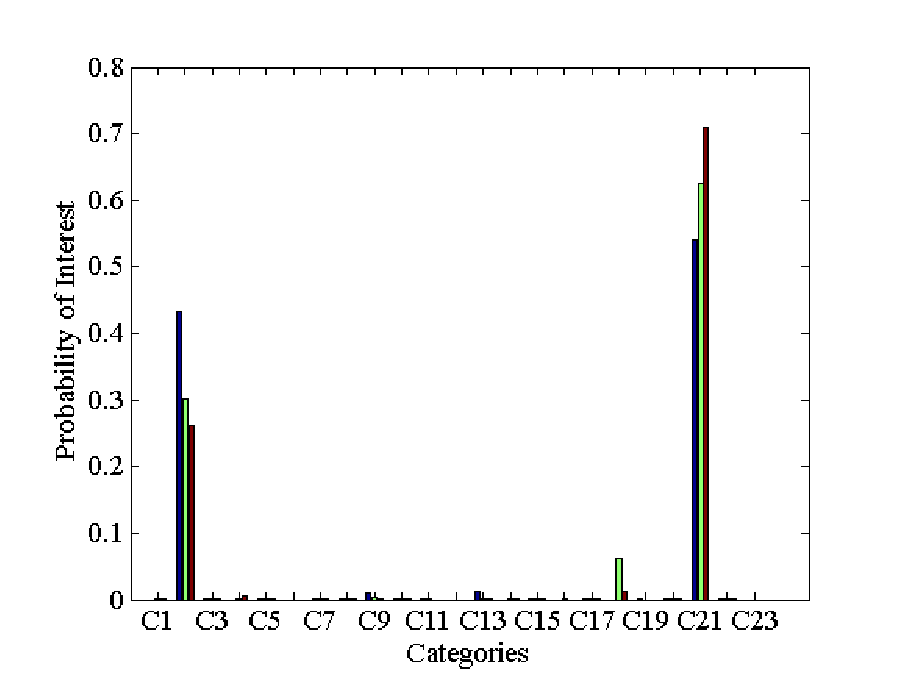
\includegraphics[width=11.5cm,height=5cm]{User2.eps} 
  \caption{Sample profile PMFs for three users from LiveLab smartphone traces.} 
       \label{fig:SampleProfile}
\end{figure}
 This key finding hinders the use of some metrics, such as Canberra
Distance and Jensen Shannon Divergence, with such sparse profiles due to the 
aforementioned infinite distance problem. 
%\par\end{flushleft}

Thus, we examine the cosine, Hellinger (HLNG), SVD and Vectorized cosine (VCOS) 
similarity metrics\footnote{Pearson correlation is not examined since it ranges 
from [-1, 1] and mapping for comparison to other metrics skew the similarity results.} 
to evaluate the pair-wise similarity for the $34$ LiveLab users,
which yields $561$ experiments. The outcomes of the four metrics
are shown, vs the experiment index, in the scatter plot depicted
in Fig.~\ref{fig:scatter}.
%
\begin{figure}[!tp]
  \centering
\includegraphics[width=12cm,height=5.3cm]{scatter.png}
%\vspace{-0.5cm}
 \caption{Metric indices for pair-wise similarity between LiveLab users.}
 \label{fig:scatter}
\end{figure}
%
First, it can be noticed from Fig.~\ref{fig:scatter} that cosine
and Hellinger similarity yield relatively higher metric values compared
to the VCOS and SVD for the same pair of users. This interesting result
confirms the intuition that temporal metrics are generally ``more
conservative'' in assessing mobile user similarity. Thus,
for a given threshold $T$ between $0$ and $1$, two users may be perceived ``similar'' using a non-temporal metric, yet, are deemed ``dissimilar'' using
a temporal metric. This is attributed to the fact that the temporal
profiles are generally more thorough since they naturally bear more details and dynamics 
than the non-temporal ones. This result is shown quantitatively in Table \ref{tab:Percentage-of-similar}.
\begin{table}
%\tabcolsep=0.05cm 
\caption{Percentage of similar users for all metrics for different similarity thresholds (T).}\label{tab:Percentage-of-similar}

\centering{}{} \label{tab:NonAndTemporal-Maj} %
\begin{tabular}{|l|l|l|l|l|l|l|l|l|l|l|}
\hline 
 & $T=$0.1 & 0.2  & 0.3  & 0.4  & 0.5  & 0.6  & 0.7  & 0.8  & 0.9  & 1\tabularnewline
\hline 
SVD  & 100  & 100  & 100  & 100  & 92.51  & 34.41  & 3.57  & 0  & 0  & 0\tabularnewline
\hline 
VCOS & 100  & 100  & 100  & 100  & 98.93  & 80.93  & 18.36  & 0.3565  & 0  & 0\tabularnewline
\hline 
Hellinger & 100  & 100  & 100  & 100  & 99.82  & 92.87  & 61.5  & 13.37  & 0  & 0\tabularnewline
\hline 
Cos & 100  & 100  & 100  & 100  & 100  & 99.47  & 97.33  & 89.13  & 59.18  & 0\tabularnewline
\hline 
\end{tabular}
\end{table}
The table shows that VCOS and SVD yield a lower percentage of similar users
than the cosine and Hellinger metrics, hence, they are more conservative. 
Second, the Hellinger metric may be perceived as a balance between both 
paradigms, since it is found to be closest to the average of the four 
metrics \cite{Mai13}. Although this demonstrates the potential of Hellinger 
similarity, it still deserves attention and analysis in future studies 
under diverse scenarios. Finally, the metrics studied and proposed here and 
the insights distilled open room for characterizing ``actual'' similarity, 
to serve as the ground truth in future work. 
%In addition, further analysis is needed to 
%contrast the HLNG and VCOS metrics to ``actual'' similarity (ground truth), 
%which is an important direction for future research.

Based on the above observations, we envision two similarity
assessment paradigms, namely macroscopic (non-temporal based) and
microscopic (temporal-based), which can serve as building blocks for 
two-stage similarity assessment.\\
\textit{Macroscopic assessment:} quantifies
similarity between two vector-based, non-temporal profiles. Evidently,
it is faster, with low-computational burden, yet, somewhat loose. Hence, it is
compelling as a ``coarse-grained'' similarity filter.\\
%This paradigm resembles getting to know a person quickly, yet, superficially.\\
\textit{Microscopic assessment:} scrutinizes similarity between two
matrix-based temporal profiles. Unlike the first paradigm, it is
more conservative in declaring similarity at the expense of more
complexity and, hence, being slower. It serves as a ``fine-grained'' 
similarity filter.

In the next section, we shift our attention to knowledge sharing in opportunistic encounters.

%**********************************************************************************
\vspace{-1.0 cm}
\section{Knowledge Sharing in Opportunistic Social Networks}
\vspace{-0.3 cm}
In the rest of the paper, we shift our attention to knowledge sharing between similar users. Our prime focus is to introduce a novel information-theoretic mathematical framework, establish fundamental limits, as opposed to designing and implementing specific knowledge sharing schemes, which constitute an interesting topic of future research. This framework lays the basis for assessing the merits of future knowledge sharing and delay-tolerant forwarding policies in opportunistic social networks.

In particular, we characterize, with the aid of information theory, the amount of knowledge a user can extract in an opportunistic encounter, coined knowledge gain (KG), and the maximum amount of knowledge available for a user in the network, coined knowledge capacity (KC). The use of modeling techniques to examine the behavior of social networks is not new. For instance, graph theory has been employed extensively to gain key insights about the behavior 
of social networks, e.g., \cite{graph1}, \cite{graph2} and \cite{graph3}. However, employing information-theoretic tools to model the knowledge gain in opportunistic, mobile social networks has not been explored before, to the best of the authors' knowledge.

%In this paper and after quantitatively assessing the similarity between mobile users given non-temporal or temporal profiles, we wish to take a look and investigate the collective knowledge available in an similarity-based opportunistic network. Modeling the user as a random variable opens ample room for using Information theory tools to measure different knowledge levels in the network. Section 1 introduces the system model in which we build our investigation upon. We then take a look about different performance metrics used to assess different forwarding schemes. We then introduce the Information-theoretic framework used to study the system at hand. We define novel concepts such as Knowledge Gain per encounter, Knowledge Capacity and Overhead per encounter in Section 2 We then introduce two profile dissemination policies namely Mine Only and Mine Plus Others'. In Section 3, we investigate two network topologies: directly connected and indirectly connected topology. We model the users using the LiveLab \cite{data} data traces. We also investigate the previously mentioned topologies in a stationary scenario and using InfoCom 2005 \cite{infocom} mobility traces in a mobile scenario.

%%%%%%%%%%%%%%%%%%%%%%%Profile Structure & Management%%%%%%%%%%%%%%%%%%%%%%%%%%%%%%%
%\section{Performance Metrics for Information Dissemination Policies}
\vspace{-0.5 cm}
\subsection{Opportunistic Network Model and Assumptions}
\vspace{-0.2 cm}
The notion of a ``network'' here, that is, nodes exchanging information, 
is established solely based on pair-wise similarity, according to Section 3.
Thus, if a group of users in an opportunistic encounter, are all dissimilar, then there is no 
network, since no knowledge sharing will follow. The scenario of interest is the one that involves a subset of similar users which triggers tips exchange. Accordingly, we focus from now on a group of nodes where all nodes are pair-wise similar.
  
We model an opportunistic encounter of $M$ similar users as a wireless adhoc network. We assume that each user is similar to all other users in the network. Each user has its own non-temporal profile vector, or multiple row vectors across the temporal dimension, modeled as a probability distribution across different categories as described in Section 3. Each user is assumed to have \textit{tips} for sharing with similar users, e.g., recommendations of an upcoming event, best seller, site visits, etc. We assume that the users leverage short-range wireless communication technologies with fixed transmission power (i.e. the circular disk model), e.g., WiFi or Bluetooth, and, hence, interference and medium access issues are resolved using these protocols.

In this section, we wish to address two fundamental questions pertaining to knowledge sharing:\\
%\begin{itemize}
{\bf 1.} For an arbitrary user $i$, what is the maximum amount of knowledge available for this user (capacity) in a given similarity-based opportunistic encounter (network)?\\
{\bf 2.} For user $i$, what is amount of knowledge gain that is achievable, i.e. the user can actually reap from similar users in the network, using a specific knowledge sharing policy?
%\end{itemize}

Towards this objective, we introduce next terminology and mathematical definitions.
%Towards this objective, we introduce next a novel, information-theoretic framework for opportunistic, mobile social networks. We first start by introducing terminology and mathematical definitions.

%The $M$ nodes happened to meet opportunistically in a place e.g. super market, museum, club, etc. In this similarity-based network, the nodes don't exchange tips unless they are deemed similar. We measure the similarity between nodes by the classic cosine similarity or a variation of this metric between the PMFs of the users. We also assume that the probabilistic characteristics of the information tips that a user has are similar to the probabilistic characteristics of the user's behaviour captured via his/her interests and experiences (same first and higher order PMFs).\\

%For this model, and using different dissemination policies we wish to assess quantitatively the performance of the different forwarding policies through different metrics that we will discuss in detail shortly.
%An effective dissemination policy would disseminate one's tips to all similar nodes in the network without incurring a large overhead given energy constraints.

%
%\subsection{Performance Metrics}
%\begin{itemize}
%\item Delivery Percentage: If there are $k$ similar users to a certain user, an optimal dissemination policy would disseminate one's tips to all the $k$ users. In general the delivery percentage is defined as the number of similar users reached $k\prime$ out of the $k$ similar users. We will show later that this resembles all users achieving their Knowledge Capacity.
%\item Average cost: the cost in our context is the average hop count the tip takes to reach the destination.
%\item Forwarding Efficiency: is defined as dividing the delivery percentage by the average cost.
%\item Knowledge Gain: will be discussed in detail in the next section.
%In the next section, we will introduce the Information-theoretic framework that will enable us to model most of the aforementioned metrics in an Information-theoretic fashion. For the next sections we will assume a mobile user $X$ is a random variable that has a discrete probability mass function (PMF). It is noted that modelling the mobile user as a random variable opens ample room for the use of Information theory as atool in characterizing notions such as Knowledge Gain, Knowledge Capacity and Overhead as follows.
%\end{itemize}
%
\vspace{-0.5 cm}
\subsection{Knowledge Capacity and Knowledge Gain}
\vspace{-0.2 cm}
In this section, we introduce two new concepts that are fundamental to the analysis that follows, namely the knowledge capacity and knowledge gain.

\begin{defn}
The Knowledge Capacity($KC_i$) is defined, for an arbitrary user $i$, as the maximum amount of knowledge that is available for user $i$ to extract from similar users in a given network.
\end{defn}

\begin{defn}
The Knowledge Gain ($KG_i$) is defined, for an arbitrary user $i$, as the amount of knowledge user $i$ can gain from similar users in a given network, using a specific knowledge sharing policy.
\end{defn}

It is straightforward to notice that $KG_i \le KC_i$ since the knowledge capacity constitutes the upper bound on the knowledge that can be reaped out of the network, irrespective of the sharing policy. Inspired by the probability distribution definition of the user profile, we argue that probability- and information-theoretic tools would prove useful for modeling and analyzing the system at hand.

Next, we introduce the formal definition of the knowledge gain per encounter. For modeling convenience, we assume that the user tips (typically stored in a table) follow a probability distribution similar to the user profile. This does not only facilitate the mathematical analysis but is also a reasonable assumption, since users tend to have more tips and recommendations in life categories they are more interested in.
%
%\begin{itemize}
%\item Knowledge Capacity for a given user (KC): defined as an upper bound on the maximum amount of new information that a user can extract from the similar users in a given network.
%\item Knowledge Gain for a given user (KG): defined as the amount of new information that a user extracted from the similar users in a given network via a specific dissemination policy. Axiomatically, the Knowledge Gain is always less than or equal to the Knowledge Capacity.
%\end{itemize}

%Since our model is probabilistic in nature (i.e the users' profiles are represented by PMFs), we use Information theory tools as one way to quantify both aforementioned notions.
%
\vspace{-0.3 cm}
\subsubsection{The Knowledge Gain per encounter}
\vspace{-0.2 cm}
We recall from information theory that the Entropy of a discrete-valued random variable $X$, denoted $H(X)$, represents a measure of the ``uncertainty'' which also represents the amount of information this random variable bears \cite{cover}. Given our assumption that the user recommendations/tips follow the same probability distribution as the user profile, tips can be modeled as a discrete random variable, $X$. Accordingly, $H(X)$ 
quantifies the amount of information (knowledge)\footnote{We use the terms Knowledge and Information interchangebly in this paper.} the user has. This model opens room for formally defining the newly introduced concepts of knowledge capacity and gain.

First, we consider a toy example of an ``opportunistic encounter'' that involves only two users within the wireless communication range of each other. The two users have tips probability distribution vectors, denoted $X$ and $Y$. Assume users $X$ and $Y$ \footnote{We abuse notation and use the tips PMFs, $X$ and $Y$, to refer to the users as well.} opportunistically meet and are deemed similar, according to Section 3. Thus, they start exchanging informative tips. Based on simple entropy relationships, depicted in the basic Venn diagram shown in Fig. ~\ref{fig:KGEncounter}, we distinguish three types of ``knowledge'' quantities (tips) that are key to our discussion: 
%
%Using our Assumption stated earlier that the probabilistic characteristics of the tips are the same as the probabilistic characteristics as his/her behaviour. We can use the information-theoretic entropy to help us quantify both Knowledge Gain and Knowledge Capacity.\\
%If we have two users $X$ and $Y$ who happen to opportunistically meet according to the similarity based opportunistic network that was described earlier and are deemed similar, they can now exchange tips.
%Using Information theory, we can quantify three important quantities as indicated in Fig. ~\ref{fig:KGEncounter}
\begin{itemize}
\vspace{-0.2 cm}
\item Tips that user $X$ has but $Y$ doesn't. ($H(X)$ excluding the intersection).
\vspace{-0.2 cm}
\item Tips that user $Y$ has but $X$ doesn't. ($H(Y)$ excluding the intersection).
\vspace{-0.2 cm}
\item Tips that both users have. (the intersection).
\end{itemize}
It is straightforward to map the first type of tips, which constitute the KG for user $X$, 
to the conditional entropy, $H(Y|X)$. Similarly, the KG for user $Y$ is given by $H(X|Y)$.
$KG(X)$ can also be written as
%
\begin{equation}
KG(X) = H(X,Y) - H(X)
\end{equation}
where $H(X,Y)$ is the joint entropy of the two random variables representing the users tips probability distributions.
%
%If $X$ and $Y$ are deemed similar and they exchange tips. From the point of view of $Y$, the new information he/she gained is the first part mentioned earlier. This part is $H(X|Y)$ i.e. the Entropy (uncertainty/information content) of user $X$ given $Y$. So, the Knowledge Gain (KG) for user $Y$ in this case is $H(X|Y)$. Along the same lines, for user $X$, $KG=H(Y|X)$.
%
%Using some basic definitions from Information theory, we can rewrite the KG for user $X$ as $H(X,Y)-H(X)$. This can be directly interpreted as the amount of joint info that both $X$ and $Y$ have minus the amount of info that $X$ has.
Finally, the third type of tips (common to both users), characterized as the mutual information $I(X;Y)$, constitutes the ``communication overhead'' since it is exchanged over the air despite the fact that it does not contribute to increasing the knowledge of $X$ or $Y$. This perfectly 
agrees with our assumption that the two users know nothing about each other, when they meet opportunistically, for the first time.
%
\begin{figure}[!tp]
  \centering
    \includegraphics[width=6.5cm ,height=5cm]{figures_png/vennSimple}
    \caption{Characterizing knowledge gain and communication verhead for users $X$ and $Y$.}\label{fig:KGEncounter}
    \end{figure}

It is worth noting that the knowledge capacity for user $X$ (or $Y$), in this toy example of two users, is equal to the knowledge gain. 
\vspace{-0.3 cm} 
\subsubsection{The Knowledge Capacity}
\vspace{-0.2 cm}
Based on the information-theoretic definitions of the KG and KC for one encounter established in the previous section, we generalize the definition to characterize the knowledge capacity for user $X_1$, without loss of generality, in an opportunistic encounter with $M-1$ other users, deemed similar to $X_1$, as follows: 
%Extending the insights that we formed about the KG quantity from the last subsection, we can now generalize the insights to get the general form for the Knowledge Capacity for a single user in a similarity-based opportunistic network of $M$ users.
%We can define the Knowledge Capacity(KC) for a single user $X_1$ as follows,
\begin{equation}
		KC(X_1) = H(X_1, X_2, X_3, ......, X_M) - H(X_1)
\end{equation}
%
%		$ | X_2, X_3, ......, X_M$ are similar to $X_1$
%\vspace{-0.6 cm}
which can be written as
\vspace{-0.2 cm}
\begin{equation}
KC(X_1) = H(X_2|X_1) + H(X_3|X_2,X_1) + .....+ H(X_M|X_{M-1}, ......, X_1)
%\nonumber
\end{equation}
%$ | X_2, X_3, ......, X_M$ are similar to $X_1$.
(3) asserts that the maximum amount of knowledge that user $X_1$ can extract from the network is simply the joint information that all users have, after removing any redundant knowledge, which is represented by the joint entropy, $H(X_1, X_2, X_3, ......, X_M)$, less the amount of information that user $X_1$ already has, that is, $H(X_1)$. It is worth noting that (3) is valid for all network topologies and is independent of knowledge sharing policies.

This powerful mathematical framework sets the stage to establish fundamental limits 
and conduct analysis of diverse opportunistic social network settings under two 
knowledge forwarding policies. This is the subject matter of the next subsection.
%Using these information theoretic tools and defining two basic information dissemination policies, we delve into different network configurations and attempt to apply the aforementioned definitions on them in order to further study them.
%%%%%%%%%%%%%%%%%%%%%%%%%%%%%%%%%%%%%%%%%%%%%%%%%%%%%%%%%%%%%%%%%%%%%%%
\vspace{-0.5 cm}
\subsection{Knowledge Sharing: Fundamental Limits and Forwarding Policies}
\vspace{-0.2 cm}
We utilize the basic definitions introduced in the previous section to establish the KC of an arbitrary user in diverse scenarios as well as characterize its KG, under two candidate knowledge sharing policies:
i) Send my tips only, or ``{\it Send Mine Only}'', whereby a user sends only his/her own 
tips to a similar, directly encountered user and ii) Forward my tips and others, or ``{\it Forward Mine Plus Others}'', whereby a user forwards own tips along with those acquired so far from others in previous encounters.

%Throughout the network model that we explained earlier, we can think of two extreme tips' exchange policies per encounter. Of course as explained earlier, the tips exchange occur only if the two users are deemed similar.
%\begin{itemize}
%\item Forward My Tips Only: or "Forward Mine Only" In this policy if the two users are similar, each one sends his/her own tips only.
%\item Forward My Tips and others: or "Forward Mine Plus Others'" In this policy if the two users are similar, each one sends his/her tips and the tips that he/she acquired from previous encounters.
%\end{itemize}
It is worth noting that these two policies are mere examples to illustrate the concept, however, other policies could be introduced and analyzed using the proposed model.
%Of course one can think of other policies or derivative policies from the previous two policies.
For instance, a user could forward his/her own tips along with a subset of others' tips based on some criteria. This gives rise to a family of knowledge sharing policies that deserves a comprehensive analysis, to assess their merits and potential trade-offs, which lies out of the scope of this work. 
%Another hybrid policy would be forward My Tips only with probability $p$ and forward mine plus others with probability $1-p$.
%Our main focus in this work is to analyse the network dynamics for the two main dissemination policies: Forward Mine Only and Forward Mine Plus Others.
%
%%%%%%%%%%%%%%%%%%%%%%%%%%%%%%%%%%%%%%%%%%%%%%%%%%%%%%%%%%%%%%%%%%%%%%%%%%%%%%%%%%%
%\section{Similarity Based Network Analysis for Different Scenarios}

Next, we shift our attention to quantifying the KC and KG achievable by the two aforementioned knowledge sharing policies, under a variety of opportunistic network configurations. In particular, we consider two connectivity scenarios, namely all nodes are within the communication range of each other (i.e. single-hop scenario) and multi-hop scenarios, where some nodes lie out of the communication range of others. In addition, we consider two network topology scenarios within an encounter, namely fixed topology (i.e. stationary or quasi-stationary users) and time-varying topology caused by the user's portability within the same area. 
%The latter case is based, in the performance analysis study, on real traces gathered throughout a conference, particularly, Infocom 2005 \cite{infocom}.  

%The network model described earlier may/may not incorporate a Mobility component. We need to study both stationary and mobile models since the nodes may be stationary or moving around in the network area. We will study both directly and indirectly connected networks as the proximity/topology of the nodes play an important role since the communication that occurs here is point to point. 
%%%%%%%%%%%%%%%%%%%%%%%%%%%%
%%Check
%%For simplicity here, we will assume all the nodes in the network are mutually similar to focus on the Knowledge related concepts.
%%%%%%%%%%%%%%%%%%%%%%%%%%%%
%
\vspace{-0.3 cm}
\subsubsection{Fixed Topology, Similarity-based Opportunistic Networks}
\vspace{-0.2 cm}
%\subsubsection{Data used for Experimentation}
%{\it A. Data used for Experimentation}\\
%For the Stationary Similarity-based Opportunistic networks and modeling the user as a Random Variable, we will be conducting our experiments using LiveLab data \cite{data} described earlier. The network consists of $20$ nodes;  $B00$, $B02$, $B03$,
%$B04$, $B05$, $B06$, $B07$, $B08$, $B09$, $B10$, $B11$, $D00$, $D01$, $D02$, $D03$, $D04$, $D05$, $D06$, $D07$ and $D08$. We shall investigate the cumulative knowledge gain after each encounter and whether the gain will reach capacity or not and how many encounters shall it take to reach capacity.
%
%\subsubsection{ Stationary, Single Hop Network:}
%%%%%%%%%%%%%%%%%%%%%%%%%%%%%%%%%%%%%%%%%%%%%%%%%%%%%%%%%%%%%%%%%%%%%%%%%%%%
\noindent {\it A. Single-hop Networks}\\
Under this setting, the users may be stationary, quasi-stationary or even mobile, yet, each
node remains one-hop away, from all other nodes, all the time. Thus, the nodes' movement does not alter the network topology, which always remains a full mesh. 
%Moreover, all nodes lie within the communication range of each other, that is, each node is a single hop away from all other nodes. 
For this setting, we can easily characterize the knowledge capacity, as in (3), and, further, prove that the knowledge gain will achieve the capacity. This is in complete agreement with intuition since any node can take turn to exchange tips with all other nodes directly reachable. Thus, ``all'' knowledge that is available for any node in this network, can be reaped. The interesting question here is: how long does it take 
to fully acquire this knowledge? It can be easily proven that it grows linearly with the network size, $M$, as confirmed by simulations which reveal interesting insights discussed in Section 4.4.
%
%Simply, since all nodes are in the same communication range of all other nodes, any node will be able to encounter any other node and extract its information, and if we assume that all nodes are mutually similar, the additive knowledge Gain will simply yield the Knowledge Capacity and this can be shown shortly.\\
The achievability result for the {\it Send Mine Only} (SMO) policy is established by the following theorem.
%
%\begin{itemize}
%\item{Stationary Directly Connected (Single Hop) Network - Forward Mine Only:}
%in this network all nodes are in each others' range and if two users are deemed similar, each user exchanges only his/her tips.
%We now present a theorem and its proof suggesting that all nodes can achieve knowledge capacity.
%
\vspace{-0.2 cm}
\begin{theorem}
For single-hop, similarity-based networks, an arbitrary node can achieve its knowledge capacity using the {\it Send Mine Only} knowledge sharing policy.
\end{theorem}
%
\vspace{-0.5 cm}
\begin{proof}
Without loss of generality, we assume that node $X_1$ encounters other nodes in an increasing order of their IDs. Under the {\it Send Mine Only} policy, 
%shown in Fig.~\ref{SSHPNet}, 
the cumulative knowledge gain for node $X_1$, $KG(X_1)$, after receiving tips from all other nodes $X_2, X_3, X_4,...., X_M$ in turn, is given by $H(X_2|X_1) + H(X_3|X_2,X_1) + .....+ H(X_M|X_{M-1}, ......, X_1)$, which is the same as $KC(X_1)$ in (4). 
%It is straightforward to notice that this summation is itself $KC(X_1)$, given in (3). 
The same argument can be applied to all other nodes in the network which proves the result.
%$H(X_1, X_2, X_3, ......, X_M) - H(X_1)= KC(X_1)$. 
%The same can also be applied to any other node and along the same lines we can prove that it can achieve its knowledge capacity.\\
%
%\begin{figure}[!tp]
%\centering
%    \includegraphics[width=8cm ,height=5.5cm]{figures_png/SSHPNet}
%    \caption{$X_1$ encounters enumerated.}\label{fig:KGEncounter}
%    \label{SSHPNet}
%\end{figure}
%
\end{proof}

\vspace{-0.4 cm}
\begin{cor}
If there is at least one node that is unreachable from the rest of the network and has at least one unique tip (that is not available at any other node), then $KG(X_1) < KC(X_1)$.
\end{cor}
\vspace{-0.2 cm}
%The proof is straightforward and is left as an exercise to the reader.\\
%
%%%%%%%%%%%%%%%%%%%%%%%%%%%%%%%%%%%%%%%%%%%%%%%%%%%%%%%%%%%%%%%%%
%\begin{theorem}
%If there is at least one node isolated from the rest of the a directly connected network that has at least one new tip (piece of information), $KG(X_1) \leq KC(X_1)$.\\
%\end{theorem}
%\begin{proof}
%%\textit{Proof:}
%Without loss of generality, we will assume that node $X_1$ will encounter other nodes in the network in an increasing order of node id and we assume a Forward Mine Only Policy. If node $X_M$ is isolated and can't be reached. So, the cumulative knowledge gain for node $X_1$, $KG(X_1)$, according to meeting nodes $X_2, X_3, X_4,...., X_{M-1}$ will be $$H(X_2|X_1) + H(X_3|X_2,X_1) + .....+ H(X_{M-1}|X_{M-2}, ......, X_1)$$ and this summation is missing the last term $H(X_M|X_{M-1}, ......, X_1)$ and since the entropy value is always greater than or equal zero so 
%$KG(X_1) <  KC(X_1) $.
%\end{proof}
%
As indicated earlier, one of the fundamental issues in our study is how long does it take a user to achieve the knowledge capacity. This is directly related to the number 
of exchanges that a user needs to perform to attain the KC. Under the {\it Send Mine Only} policy and assuming that each node has at least one unique tip to contribute to the knowledge in the network, then it is straightforward to show that the worst-case number of exchanges needed for an arbitrary node to attain the KC is simply $(M-1)$, that is, $O(M)$.
%%%%%%%%%%%%%%%%%%%%%%%%%%%%%%%%%%%%%%%%%%%%%%%%%%%%%%%%%%%%%%%%%%%%%%%%%%%%%
%\item{Stationary Directly Connected (Single Hop) Network - Forward Mine Plus Others':}

Next, we shift our attention to quantify the KG and time-to-achievability of single-hop networks, under the {\it Forward Mine Plus Others} (FMPO) sharing policy. Thus, a user shares not only its own tips but also tips collected from previous encounters, denoted by the subscript $p$. We prove in the following theorem that the knowledge capacity is also achievable using the FMPO policy.
%in this network all nodes are in each others' range and if two users are deemed similar, each user exchanges his/her tips and the tips he/she has extracted from previous encounters. We model previous tips by subscript $p$.

%For the Stationary Directly Connected (Single Hop) network, and using Mine Plus Others' forwarding scheme, we can also show that any node can achieve the Knowledge Capacity.\\
%\textit{Example:}In a network of $4$ nodes ($X_1, X_2, X_3, X_4$), if we use a Mine Only forwarding scheme, $X_1$ will have to make $3$ encounters with $X_2, X_3$ and $X_4$ to reach its Knowledge Capacity. If we use a Mine Plus Others' forwarding scheme as shown in Fig. $X_1$ will reach the capacity in $2$ encounters.\\
%
\vspace{-0.2 cm}
\begin{theorem}
For single-hop similarity-based networks, an arbitrary node achieves the knowledge capacity using the FMPO knowledge sharing policy.
\end{theorem}
%
\vspace{-0.5 cm}
\begin{proof}
We proceed along the lines of Theorem 1 and give an outline of the proof due to space limitations. Without loss of generality, we assume that node $X_1$ encounters all other nodes in an increasing order of their node IDs. Thus, $KG(X_1)$ based on encountering nodes $X_2, X_3, X_4,...., X_M$ in turn, is given by
\begin{equation}
KG(X_1) = H(X_2, \vec{X_{2p}}|X_1) + H(X_3, \vec{X_{3p}}|X_2, \vec{X_{2p}}, X_1) + H(X_4, \vec{X_{4p}}|X_3, \vec{X_{3p}}, X_2, \vec{X_{2p}}, X_1)+.....
\nonumber
\end{equation} 
\begin{equation}
\hspace*{-6 cm} + H(X_M, \vec{X_{Mp}}|X_{M-1}, \vec{X_{(M-1)p}} ,......, X_1)
\end{equation}
\noindent where $\vec{X_{ip}}$ captures the previous encounters of node $X_i$. It can 
be shown that each joint entropy term in (5) can be expanded, 
e.g., $H(X_2, \vec{X_{2p}}|X_1)$ becomes $H(X_2|X_1) + H(\vec{X_{2p}}|X_2, X_1)$, where 
the latter term (previous encounter tips of a node) would be redundant in some cases (acquired from earlier encounters) and, hence, contributes zero to the KG. This, in turn, reduces (5) to the KC in (4) and proves the result.
%This reduces to the  KC in (3) and proves the result.
\end{proof}
%
It should be noted that once the conditioning, in the conditional entropy terms in the RHS, accommodates all nodes in the network, the incremental gain becomes zero and the node achieves its knowledge capacity. In essence, the role of the previous encounters (prevails in the conditional entropy terms) is the prime contributor to the FMPO policy attaining the KC faster, compared to the SMO policy. Apparently, this does not come 
for free since there is a fundamental trade-off between the cumulative KG after a number of exchanges and the associated overhead which warrants attention in future research, especially in multi-hop networks. We prove next that the communication overhead of FMPO is greater than or equal to SMO, in single-hop networks.
%
\vspace{-0.2 cm}
\begin{theorem}
For single-hop networks, the communication overhead under FMPO is greater than or equal to SMO.
\end{theorem}
%
\vspace{-0.5 cm}
\begin{proof}
Assume two users, $X$, $Y$, encounter each other. Denote the vector of previous encounters for $X$ and $Y$ by $\vec{X_p}$ and $\vec{Y_p}$, respectively.

Under the SMO policy, the communication overhead that $X$ incurs is the common knowledge (mutual information) between what $X$ sends (which is its knowledge only) and $Y$'s 
knowledge so far which is given by 
\begin{equation}
OH(X)_{SMO}=I(X;Y,\vec{Y_p}).
\label{overheadX}
\end{equation}
Similarly, the communication overhead from the perspective of user $Y$ is $OH(Y)_{SMO}=I(Y;X,\vec{X_p})$.

Under FMPO, the communication overhead is the same for both users, $X$ and $Y$, and is given by
\begin{equation} 
OH(X)_{FMPO}=OH(Y)_{FMPO}=I(X,\vec{X_p};Y, \vec{Y_p}).
\label{overheadXY}
\end{equation}

From information theory, the mutual information between two random variables $A$ and $B$ can be written as
\begin{equation} 
I(A;B)=H(A) + H(B) - H(A,B).
\label{mutInfoEqn}
\end{equation}
%\vspace{-0.4 cm}
Applying ~\eqref{mutInfoEqn} on ~\eqref{overheadX} yields
\begin{equation}
OH(X)_{SMO}= H(X)+H(Y,\vec{Y_p})-H(X,Y,\vec{Y_p}).
\label{Eqn.4}
\end{equation}
Applying ~\eqref{mutInfoEqn} on ~\eqref{overheadXY} yields
\begin{equation}
OH(X)_{FMPO}=OH(Y)_{FMPO}= H(X,\vec{X_p})+H(Y,\vec{Y_p})-H(X,\vec{X_p},Y,\vec{Y_p}).
\label{Eqn.3}
\end{equation}
Subtracting ~\eqref{Eqn.4} from ~\eqref{Eqn.3} yields 
\begin{equation}
OH(X)_{FMPO}-OH(X)_{SMO}=H(X,\vec{X_p})-H(X)-H(X,\vec{X_p},Y,\vec{Y_p})+H(X,Y,\vec{Y_p})
%H(Y,\vec{Y_p})-H(Y)-H(X,\vec{X_p},Y,\vec{Y_p})+H(X,\vec{X_p},Y).
\label{Eqn.5}
\end{equation}
Since $H(A,B) = H(A) + H(B|A) = H(B) + H(A|B) $, ~\eqref{Eqn.5} could be re-written as
\begin{equation}
OH(X)_{FMPO}-OH(X)_{SMO}=H(X)+H(\vec{X_p}|X)-H(X)-[H(\vec{X_p}|X,Y,\vec{Y_p})+H(X,Y,\vec{Y_p})] + H(X,Y,\vec{Y_p})
\nonumber
\end{equation}
which reduces to 
\begin{equation}
OH(X)_{FMPO}-OH(X)_{SMO}=H(\vec{X_p}|X)- H(\vec{X_p}|X,Y,\vec{Y_p})
\label{lasteqn}
\end{equation}
\begin{equation}
\hspace*{0.6 cm} \ge 0
\label{ineq}
\end{equation}
where the inequality in~\eqref{ineq} follows since conditioning reduces entropy. This proves the result.
\end{proof}
%
%\vspace{-0.3 cm}
%\noindent \textbf{Example 1.} This example illustrates the KC achievability speedup under FMPO. Consider a network of $4$ users, $X_1, X_2, X_3, X_4$, going through two encounters as shown in Figs.~\ref{fig:SSHP(MO1)}(a) and (b), respectively. The two figures show the knowledge at a node before exchange (KBE) and the knowledge after exchange (KAE). It can be noticed from Fig.~\ref{fig:SSHP(MO1)}(b) that all nodes would reach their KCs after, only, two encounters, as opposed to $M-1$ encounters (three in this scenario) under the {\it Send Mine Only} (SMO) policy.
%
%\vspace{-0.3 cm}
%\begin{figure}[!bp]
%\centering
%    \includegraphics[width=8cm ,height=5cm]{figures_png/SSHP(MO1)}
%    \hspace {1 cm} \includegraphics[width=8cm ,height=5cm]{figures_png/SSHP(MO2)}
%\centerline{(a) \hspace{9 cm} (b)}
%    \caption{Illustrating the KC achievability speedup using FMPO: (a) 1st encounter, (b) 2nd encounter.}\label{fig:SSHP(MO1)}
%    \label{SSHP(MO1)}
%\end{figure}
%
%
%
%\begin{figure}[!bp]
%\centering
%    \includegraphics[width=8cm ,height=5.5cm]{figures_png/SSHP(MO2)}
%    \caption{A scenario for encounters (Second Step).}\label{fig:SSHP(MO2)}
%    \label{SSHP(MO2)}
%\end{figure}
%\vspace{-0.2 cm}
%\begin{figure}[htpb]
%\epsfysize 2.5in
%\centerline{\epsfbox{example2.eps} \epsfysize 2.5in \epsfbox{example3.eps}}
%\centerline{(a) \hspace{7.6 cm} (b)}
%\centerline{\epsfysize 2.5in \epsfbox{example4.eps}}
%\centerline{(c)}
%\vspace{-0.3 cm}
%\caption{Three Interference Scenarios with ten 8x8 MIMO links: (a) Low Interference, (b) Medium Interference, (c) High Interference}
%\end{figure}

%On the other hand, if we each node uses a Forward My Tips and others dissemination policy and if we assume that the system of the nodes will be exchanging tips for a while before a new node enters the network environment, then we have two extreme cases as follows.\\
%In the best case, where the new entering node named $X$ meets a node that has gathered all the tips in the system named $Y$, then the number of exchanges that $X$ needs to attain capacity is one, hence a complexity of $O(1)$.\\
%On the other hand, the worst case scenario is simply when no enough exchanges are done before node $X$ enters the system and this leads to the Mine plus others scheme falling back to the Mine Only scheme and the number of exchanges needed by $X$ to attain capacity will be $O(N)$.
%
%%%%%%%%%%%%%%%%%%%%%%%%%%%%%%%%%%%%%%%%%%%%%%%%%%%%%%%%%%%%%%%%%%%%%%%%%%%%%%%%
%\subsubsection{Stationary Indirectly Connected Network:} 
\vspace{-0.2 cm}
\noindent {\it B. Fixed Topology Multi-hop Networks}\\
Under this setting, the network topology is time-invariant, however, not all nodes are 
directly reachable from each other, i.e. multi-hop paths will be followed for exchanging 
some tips. In this case, the role of the knowledge sharing policy stands out and affects 
whether a user can/cannot attain the KC.
%
%in this kind of network, not all nodes are in the same communication range of each other. If we take node $X_1$ for example, then in this kind of network it will have a subset of the $M$ nodes, say $N$ where $N<M$, in the same communication range or one hop away and the other $M-N$ nodes not reachable by $X_1$.\\
%Here the information dissemination policy plays an important role in whether or not a node attains the Knowledge Capacity.
%
%\begin{itemize}
%\item{Stationary Indirectly Connected (Multi-Hop) Network - Forward Mine Only:}

Next, we quantify the performance, and trade-offs, of the two aforementioned knowledge sharing policies, namely SMO and FMPO. In case of
%in this network shown in Fig.~\ref{SMHPNet}
SMO, the knowledge gain achieved by node $X_1$ is limited by the neighborhood size, $N$<$M$. This renders the KG under this policy strictly less than the KC for multi-hop networks. The following theorem formally establishes this result.
\vspace{-0.2 cm}
\begin{theorem}
For fixed topology, multi-hop, similarity-based networks, the {\it Send Mine Only} knowledge sharing policy will not attain capacity, that is, $KG(X_1)<KC(X_1)$ iff $N<M$.
\end{theorem}
%\textit{Proof:}\\
%
\vspace{-0.4 cm}
\begin{proof}
Without loss of generality, we assume node $X_1$ communicates with other nodes in an increasing order of their IDs. The cumulative knowledge gain for node $X_1$, $KG(X_1)$, according to exchanges with neighbors $X_2, X_3, X_4,...., X_{N}$ is given by $H(X_2|X_1) + H(X_3|X_2,X_1) + .....+ H(X_{N}|X_{N-1}, ......, X_1)$. It is worth noting that the summation of positive conditional entropy terms is limited to $N<M$ nodes. It misses other positive terms involving the $M-N$ non-neighbors to $X_1$. Hence, it directly follows that $KG(X_1)<KC(X_1)$, which proves the result.
%
%and this summation is missing the terms $H(X_{N+1}|X_{N}, ......, X_1)$ till $H(X_{M}|X_{M-1}, ......, X_1)$ and since these terms are entropy terms whose values are always greater than or equal zero so.
\end{proof}
%
\vspace{-0.5 cm}
It is worth noting that the special case of $N=M$, for all nodes, reduces to the single-hop network case where we have shown in Section 4.3.1.A that the KC is achievable under both knowledge sharing policies.
%
%The situation differs for example for any node that has all nodes in its range i.e., $N=M$. For this node, capacity will be achieved (all missing terms from the last proof will be added and the gain reaches capacity). 
%
An interesting, and somewhat surprising, insight which will be discussed later, is that nodes mobility can be leveraged to achieve the knowledge capacity, even if $N<M$.

%\begin{figure}[!tp]
%\centering
%    \includegraphics[width=8cm ,height=5.5cm]{figures_png/SMHP(MO)}
%    \caption{Fixed Topology Multi-Hop Network.}\label{fig:SMHP(MO)}
%    \label{SMHPNet}
%\end{figure}
%===========================================================================================
%\item{Stationary Indirectly Connected (Multi Hop) Network - Forward Mine Plus Others':}

In the rest of this section, we focus on the performance of the FMPO knowledge sharing policy 
for fixed topology multi-hop networks. As expected, forwarding others tips opens room for a node to achieve its KC, even when $N<M$. The following theorem formally establishes this result. 
%we now study this network using a Forward Mine Plus Others' policy. If we assume multiple encounters with the same node is allowed and the neighboring nodes for $X_1$ collected the knowledge of non-neighbouring nodes for $X_1$, then $X_1$ can attain its knowledge capacity. We now present this in the next theorem.
%
\vspace{-0.2 cm}
\begin{theorem}
For fixed topology, multi-hop, similarity-based networks, an arbitrary node can achieve the knowledge capacity using the FMPO knowledge sharing policy.
\end{theorem}
%
%\textit{Proof:}
\begin{proof}
Without loss of generality, we assume that each node starts off with its own knowledge only and $X_1$ encounters other nodes in an increasing order of their IDs, while other neighbors have pair-wise encounters with other nodes in the network. The cumulative knowledge gain for node $X_1$, $KG(X_1)$, after communicating with neighboring nodes $X_2, X_3, X_4,...., X_N$ is given by
\vspace{-0.2 cm}
\begin{equation}
KG(X_1)=H(X_2,|X_1) + H(X_3, \vec{X_{3p}}|X_2,X_1) + H(X_4, \vec{X_{4p}}|X_3, \vec{X_{3p}}, X_2,X_1)+.....
\nonumber
\end{equation}
\begin{equation}
\hspace*{-4.3 cm} + H(X_N, \vec{X_{Np}}|X_{N-1}, \vec{X_{(N-1)p}} ,......, X_1) 
\end{equation}
where $\vec{X_{ip}}$ represents the previous encounters of node $i$. At this point, two cases arise. First, if the previous encounters include ``forwarded'' tips from all non-neighboring nodes, namely $X_{N+1}, X_{N+2}, ......, X_M$, then it can be shown that the cumulative knowledge gain of $X_1$ is given by
%
\vspace{-0.4 cm}
\begin{equation}
KG(X_1)=H(X_1, X_2, X_3, ......, X_M) - H(X_1)= KC(X_1) 
\end{equation} 
%
\noindent which attains the $KC(X_1)$. On the other hand, if the previous encounters do not cover tips from non-neighbors, then this implies that node $X_1$ needs more time to attain $KC(X_1)$, possibly via revisiting neighbors that it has already visited to acquire the missing knowledge from nodes out of its communication range, until it eventually reaches capacity. 
%It should be noted that once the conditioning, in the conditional entropy terms in the RHS, accommodate all in the network, the incremental gain becomes zero and the node achieves its knowledge capacity.
%Of course once the right hand side of the given sign has the full list of the nodes in the network, the added gain will be zero and the node will have reached its Knowledge Capacity.
This proves the theorem.
\end{proof}
%\end{itemize}

%On the contrary, if the dissemination policy used in this network is Forward Mine Plus Others we can find best and worst cases scenarios.
%The best case for this situation happens when the $N$ neighbouring nodes have the knowledge (tips) of the non-neighbouring nodes. If that is the case and through using the Mine plus others policy, $X$ could attain the Knowledge Capacity.
%The worst case for this situation happens when the $M-N$ non neighbouring nodes for $X$ can't be reached by the $N$ neighbouring nodes and thus this case falls back to the Mine Only strategy in the last paragraph.
%The average case naturally happens when some of the non-neighbouring nodes are achievable and some aren't and in this case also $X$ can't attain Knowledge Capacity as well.
%%%%%%%%%%%%%%%%%%%%%%%%%%%%%%%%%%%%%%%%%%%%%%%%%%%%%%%%%%%%%%%%%%%%%%%%%%%%%%%%%%%%%5
%\subsubsection{LiveLab Results for Stationary Similarity-based Opportunistic Network }
\vspace{-0.5 cm}
\subsection{User Traces and Performance Results}
%\section{Real User Traces and Performance Results}
\vspace{-0.2 cm}
In this section, we back our theoretical findings with numerical results based on 
smartphone traces for user profiles \cite{data} and real-life user mobility traces, gathered at Infocom 2005 \cite{infocom,diot}.
\vspace{-0.3 cm}
\subsubsection{Single-hop Similarity-based Networks}
%\subsection{Fixed Topology, Single-hop Similarity-based Networks}
\vspace{-0.2 cm}
%
%After describing the different topologies for the similarity-based Opportunistic Network under investigation, we now present the results after incorporating 
%
In this section, we rely on real-life traces, either for user behavior or mobility. For user behavior, we utilize digital footprint traces for $20$ smartphone users from the LiveLab project \cite{data}. In this section, the users are assumed stationary, or quasi-stationary, and, hence, the network topology is a time-invariant full mesh. In order to quantify the knowledge capacity and gain for an arbitrary user in this network, we need to pre-process the huge amount of data in two steps. First, we compute the joint probability mass function for the 20 users under investigation over a period of six months, from September 2010 to February 2011. Thus, we monitor the users' activities categorized under $24$ categories\footnote{The 24th category captures the case when the smartphone is off or not running any application.}, each second, for six months and record their concurrent activities. Afterwards, we divide by the total duration of the six months to get the joint PMF. Next, we show the cumulative knowledge gain increase as the node under investigation encounters more nodes over time.
%===========================================================================================================
%\begin{itemize}
%\item Results for Stationary Directly Connected (Single-Hop)- Mine Only Network:

First, we present the performance results for a single-hop network under the 
SMO knowledge sharing policy. For the network of $M=20$ nodes discussed earlier, an 
arbitrary user can achieve the knowledge capacity in $M-1=19$ exchanges. This is shown in Fig.~\ref{fig:B00_SSHOP)} for three arbitrary users, namely $B00$, $B04$ and $D03$. It is also worth noting that the cumulative knowledge gain is a non-decreasing function with time. On the other hand, the knowledge capacity is shown as a horizontal solid line that is generally different from one node to another.
%
\begin{figure}[!tp]
\centering
    \includegraphics[width=10cm ,height=5.6cm]{figures_png/Fig5}
%    \includegraphics[width=8.1cm ,height=5.6cm]{figures_eps/B02_SSHOP}
%\centerline{(a) \hspace{9 cm} (b)}
%\includegraphics[width=8.1cm ,height=5.6cm]{figures_eps/D00_SSHOP}
%\centerline{(c)}
    \caption{Cumulative knowledge gain for three users in a fixed topology single-hop network under SMO.}\label{fig:B00_SSHOP)}
\end{figure}
%
%\begin{figure}[!tp]
%\centering
%    \includegraphics[width=12cm ,height=7cm]{figures_eps/B02_SSHOP}
%    \caption{Cumulative knowledge gain for user B02 in a fixed topology single-hop network under (SMO).}\label{fig:B02_SSHOP)}
%\end{figure}
%\begin{figure}[!tp]
%\centering
%    \includegraphics[width=12cm ,height=7cm]{figures_eps/D00_SSHOP}
%    \caption{Cumulative knowledge gain for user D00 in a fixed topology single-hop network under (SMO).}\label{fig:D00_SSHOP)}
%\end{figure}
%================================================================================================================
%\item Results for Stationary Directly Connected (Single-Hop)- Mine Plus Others' Network:

Next, we shift our attention to the same network setting, yet, employing the FMPO policy.
Based on Theorem 2, we show that, for this type of networks, all nodes achieve the knowledge capacity using the FMPO policy, yet, faster than SMO, i.e. in less encounters due to sharing the tips of others. This valuable insight is confirmed for users $B00$, $B04$ and $D03$ in Fig.~\ref{fig:B00_SSHOP(MO)}.
%
\begin{figure}[!bp]
\centering
    \includegraphics[width=10cm ,height=5.6cm]{figures_png/Fig6}
%    \includegraphics[width=8.1cm ,height=5.6cm]{figures_eps/B04_SSHOP_MO.eps}
%\centerline{(a) \hspace{9 cm} (b)}
%  \includegraphics[width=8.1cm ,height=5.6cm]{figures_eps/D03_SSHOP_MO.eps}
%  \centerline{(c)}
    \caption{Cumulative knowledge gain for three users in a fixed topology single-hop network under FMPO.}\label{fig:B00_SSHOP(MO)}
\end{figure}
%\begin{figure}[!bp]
%\centering
%    \includegraphics[width=12cm ,height=7cm]{figures_eps/B04_SSHOP_MO.eps}
%    \caption{Cumulative knowledge gain for user B04 in a fixed topology single-hop network under FMPO.}\label{fig:B04_SSHOP(MO))}
%\end{figure}
%    \begin{figure}[!bp]
%\centering
%    \includegraphics[width=12cm ,height=7cm]{figures_eps/D03_SSHOP_MO.eps}
%    \caption{Cumulative knowledge gain for user D03 in a fixed topology single-hop network under FMPO.}\label{fig:D03_SSHOP(MO))}
%\end{figure}
%=================================================================================================================
%\item Results for Stationary Indirectly Connected (Multi-Hop)- Mine Only Network: 
\vspace{-0.4 cm}
\subsubsection{Fixed Topology, Multi-hop Similarity-based Networks}
%\subsection{Fixed Topology, Multi-hop Similarity-based Networks}
\vspace{-0.2 cm}
In this section, we shift our attention to fixed topology, multi-hop networks 
where we study the cumulative knowledge gain behavior under the SMO and FMPO knowledge sharing policies.

As indicated earlier, and shown formally in Theorem 4, achieving the KC of an arbitrary node using SMO is fundamentally limited by the single-hop neighborhood size of this node, denoted $N$.
%For this kind of network, any node is limited in achieving the capacity by the neighborhood size. 
For instance, we generate $20$ randomly generated topologies of uniformly distributed users whereby each user has 6-7 single-hop neighbors, out of $20$ nodes, on the average. Thus, $B00$ 
%, namely $B03$, $B05$, $B09$, $B11$, $B07$, $D01$, $D03$, $D05$, 
does not achieve the KC for it in this network, as established in Theorem 4 and shown here using real smartphone user behavior traces in Fig.~\ref{fig:B00_SMHOP)}. Thus, the maximum KG node $B00$ can achieve is only 43\% of its KC. Similarly, users $B06$ and $D00$ have single-hop neighbors strictly less than $M=20$ and, hence, cannot achieve their respective KCs. 
%This is shown numerically in Fig.~\ref{fig:B00_SMHOP)}.
%
\begin{figure}[!bp]
\centering
 \includegraphics[width=10cm ,height=5.6cm]{figures_png/Fig7}
% \includegraphics[width=8.1cm ,height=5.6cm]{figures_eps/B06_SMHOP}
% \centerline{(a) \hspace{9 cm} (b)}
% \includegraphics[width=8.1cm ,height=5.6cm]{figures_eps/D00_SMHOP}
% \centerline{(c)}
    \caption{Cumulative knowledge gain for three users in a fixed topology multi-hop network under SMO.}\label{fig:B00_SMHOP)}
\end{figure} 
%\begin{figure}[!bp]
%	\centering
%     \includegraphics[width=12cm ,height=7cm]{figures_eps/B06_SMHOP}
%    \caption{Cumulative knowledge gain for user B06 in a fixed topology multi-hop network under SMO.}\label{fig:B06_SMHOP)}
%\end{figure}
%\begin{figure}[!bp]
%	\centering
%     \includegraphics[width=12cm ,height=7cm]{figures_eps/D00_SMHOP}
%    \caption{Cumulative knowledge gain for user D00 in a fixed topology multi-hop network under SMO.}\label{fig:D00_SMHOP)}
%\end{figure}
    
%\item Results for Stationary Indirectly Connected (Multi-Hop)- Mine Plus Others' Network: 
In the rest of this section, we analyze the KG and KC performance of the FMPO policy in multi-hop topologies. In this case, the FMPO policy is expected to overcome the limited neighborhood problem due to sharing others' knowledge (tips) and, hence, the nodes could achieve the knowledge capacity as proven in Theorem 5. The results here are based on the $20$ randomly generated topologies discussed earlier.  
%The first layer contains node $B00$, the second layer contains ten nodes and the third layer contains nine nodes. 
%It is assumed that a node in one tier could only encounter nodes in the directly lower or higher tier. 
The cumulative knowledge gains for users $B00$, $B06$ and $D00$ are depicted in Fig.~\ref{fig:B00_SMHOP_MO)}. We notice that the KC is achievable for the three shown users after $8$, $9$ and $10$ encounters, respectively.
%
  \begin{figure}[!bp]
	\centering
     \includegraphics[width=10cm ,height=5.6cm]{figures_png/Fig8}
%     \includegraphics[width=8.1cm ,height=5.6cm]{figures_eps/B06_SMHOP_MO}
% \centerline{(a) \hspace{9 cm} (b)}
%     \includegraphics[width=8.1cm ,height=5.6cm]{figures_eps/D00_SMHOP_MO}
%     \centerline{(c)}
    \caption{Cumulative knowledge gain for three users in a fixed topology multi-hop network under FMPO.}\label{fig:B00_SMHOP_MO)}
\end{figure}
%\begin{figure}[!bp]
%	\centering
%     \includegraphics[width=12cm ,height=7cm]{figures_eps/B06_SMHOP_MO}
%    \caption{Cumulative knowledge gain for user B06 in a fixed topology multi-hop network under FMPO.}\label{fig:B06_SMHOP_MO)}
%\end{figure}  
%\begin{figure}[!bp]
%	\centering
%     \includegraphics[width=12cm ,height=7cm]{figures_eps/D00_SMHOP_MO}
%    \caption{Cumulative knowledge gain for user D00 in a fixed topology multi-hop network under FMPO.}\label{fig:D00_SMHOP_MO)}
%\end{figure}
%
%\end{itemize}
%==================================================================================================
\vspace{-0.6 cm}
\subsubsection{Time-varying Topology (Mobile) Similarity-based Networks}
%\subsection{Time-varying Topology (Mobile) Similarity-based Networks}
\vspace{-0.2 cm}
%\subsubsection{User Profile and Mobility Traces}
%
\noindent {\it A. User Profiles and Mobility Traces}\\
%\subsubsection{User Profile and Mobility Traces}
%
After an extensive search for mobile user traces on publicly available data repositories, e.g., CRAWDAD \cite{infocom,diot} and the alike, we did not find traces that include both, user behavior and mobility patterns. Moreover, most of the mobility traces are university campus WiFi access patterns as opposed to user encounters. In order to proceed with the performance evaluation based on real data, we resort to jointly leveraging traces from 
different data sets, for the profiles and mobility. As for user profiles, they are distilled 
and constructed based on the LiveLab project data \cite{data} described earlier. On the other hand, user mobility traces are based on a ``conference encounter'' data, namely Infocom 2005 \cite{infocom,diot}. Towards this objective, we project the user profile probability distributions, constructed from the LiveLab data, on the Infocom user mobility traces. For the Infocom 2005 experiment, the data set is relatively small whereby participants are $50$ attending the student workshop. Nevertheless, it constitutes a reasonably sized set for our performance evaluation purposes. The students were given iMotes on March $7^{th}$, $2005$ between lunch time and $5$ pm and collected on March 10th, 2005 in the afternoon. Two iMotes were lost while seven did not deliver useful data due to an accidental hardware reset. Contacts with these nine iMotes were discarded from the traces of others to avoid any effect on the results. 
The first six hours are discarded since they were attending the same workshop. We consider the contacts of $20$ nodes only to match the number used from the LiveLab user profiles data. Thus, we associate the profiles of $20$ randomly chosen users from the LiveLab data set 
%$B00$, $B02$, $B03$, $B04$, $B05$, $B06$, $B07$, $B08$, $B09$, $B10$, $B11$, $D00$, $D01$, $D02$, $D03$, $D04$, $D05$, $D06$, $D07$ and $D08$ 
to the mobility traces of $20$ iMotes from Infocom 2005 and monitor them for half a day. This enables us to conduct our knowledge sharing analysis and collect the sought performance results.
%quantify the cumulative knowledge gain after each encounter and whether the gain will reach capacity or not and how many encounters would it take until achieving capacity.

Despite the fact that user profile and mobility traces are brought from two totally independent data sets, we find it a very useful attempt towards evaluating our policies, due to the lack of the sought data in the public domain. This constitutes a strong motivation for the mobile networking and computing community to focus on the social dimension as well as the mobility and wireless connectivity dimensions, which already have several data sets in the public domain.
%
%For mobile similarity-based opportunistic networks and modeling the user as a Random Variable, 
%we will be conducting our experiments using LiveLab data \cite{data} described earlier and InfoCom 2005 mobility traces. We project the PMFs from LiveLab data onto the user mobility traces \cite{infocom} from the conference IEEE Infocom 2005. 
%
%==================================================================================================
%\subsubsection{Mobile directly Connected (Single Hop) Network:}
%
%\noindent {\it B. Mobile, Single-hop Networks}\\
%Despite the fact that this is a mobile network, it is easy to notice 
%that it is not much different from fixed topology networks, since nodes remain one-hop away from each other all the time, in both cases.

%If we think thoroughly about this kind of network, we will find that all nodes in the network are one hop away from each other. Even when the nodes move, they are still in each other's range. 
%Accordingly, nodes' mobility in this case does not have an effect on the KG and KC at all. 
%Each time a node wants to exchange information with other nodes, he/she will poll to see what nodes are in its range and the result will be that all nodes are in its range. 
%This is the same case of the Stationary directly Connected (Single Hop) Network with its two cases; Forward Mine Only and Forward Mine Plus Others'. So, the same results will be achieved as in the last section.\\ 
%=================================================================================================
%
%\subsubsection{ Mobile Indirectly Connected (Multi Hop) Network:}
\vspace{0.1 cm}
\noindent {\it B. Time-varying Topology Multi-hop Networks}\\
%\subsubsection{Time-varying Topology, Multi-hop Networks}
In this section, we quantify the knowledge capacity and gain of time-varying topology (mobile) multi-hop networks, under the two sharing policies. 
%Recall that the case of mobile, single-hop networks simply reduces to fixed topology, single-hop networks studied in Section 3.3.1.A.
Intuitively, users' mobility would play a key role in whether a node can achieve its 
KC and, if so, how much time this would incur. 
%We evaluate the KG and KC performance for the SMO and FMPO policies, using the LiveLab profile traces and Infocom 2005 mobility traces.
%
%As a result, Mobility is a factor in achieving/not achieving knowledge capacity and how fast a node could achieve this capacity. 
%We investigate this kind of network for the two cases; Mine Only and Mine Plus Others' using Infocom traces. 
%
The gathered results are shown in Table ~\ref{tab:Infocom}. We compare the KG acquired by 
sample nodes using SMO in two cases, namely the stationary case where a snapshot is taken at time $t=0$ and the mobile case over half a day. At time $t=0$, 
all nodes, except for node $B07$, are disconnected yielding KG of zero. Node $B07$ is initially connected to $D06$ and reaps a KG of 0.64 as shown. The intriguing observation here is that mobility does help some nodes to approach the knowledge capacity. On the other hand, some nodes, e.g., $B06$, do not benefit from mobility since they remain disconnected throughout the 
experiment time span. This insight agrees with intuition since the mobility patterns of some nodes could assist them in encountering the ``knowledge hot spots'' of the network.
%, i.e., the nodes who offer them the highest knowledge gain 
On the other hand, the mobility of other nodes could give rise to encounters with very slim/no 
KG benefits, e.g. nodes $B02$ and $B06$. Finally, we highlight that FMPO achieves no less KG than SMO, over the same period of time, which agrees with our theoretical findings.

Extensive studies of user encounter patterns in campus WLANs, e.g., \cite{hsu,diot}, have shown that, on the average, a user encounters only 2\% of the population in a month and pointed out the heavy clustering of a user's behavior (spending 90\% of their online time within only five APs (out of ~600). In the following theorem, we establish the proof based on an ideal mobility model guaranteeing encounter with all other nodes, which may not be valid
for a whole campus scenario based on \cite{hsu}. Nevertheless, for local encounters and mobile communities, the encounter ratio tends to be quite high (vs. 2\% for the whole population) 
and our model is likely to be valid for realistic mobility scenarios.

Based on the seminal work on the effect of mobility on the throughput and delay in wireless ad hoc networks \cite{elgamal}, the following theorem proves that the knowledge capacity in mobile, delay-tolerant, multi-hop social networks is always achievable, under idealistic assumptions and loose delay constraints. Those assumptions guarantee that an arbitrary node will encounter all other nodes in the network, almost surely.
%, or at least, the minimum set of nodes who bear the knowledge capacity, for that node, in the network. 
Nevertheless, characterizing the realistic mobility scenarios and conditions under which the KG of a node is improved by mobility is an interesting subject of future research.
%have ergodic mobility patter, i.e. , and loose delay constraints. 
%
%We can prove that for this kind of network, if the nodes have an ergodic mobility pattern, capacity could be achieved.
%
\vspace{-0.2 cm}
\begin{theorem}
For a time-varying topology, multi-hop, similarity-based network, an arbitrary node achieves its knowledge capacity, almost surely, in case each 
node moves according to an independent 2-dimensional random walk in a fixed 
area and under loose delay constraints.
%For a time-varying topology, multi-hop network, the if the nodes have an ergodic mobility pattern, capacity could be achieved.
\end{theorem}
\vspace{-0.5 cm}
\begin{proof}
In case of loose delay constraints and independent 2-dimensional random walks, an arbitrary node will encounter all other nodes in the network, almost surely (follows from Lemma 6 in \cite{elgamal}).
%An ergodic mobility model means that every node will encounter every other node. 
Hence, without loss of generality, we assume that node $X_1$ encounters all nodes in an increasing order of their node IDs. Under SMO, the cumulative knowledge gain for node $X_1$, $KG(X_1)$, based on encountering nodes $X_2, X_3, X_4,...., X_M$ is the same as (4).
%\vspace{-0.2 cm} 
%\begin{equation}
%KG(X_1)=H(X_2|X_1) + H(X_3|X_2,X_1) + .....+ H(X_M|X_{M-1}, ......, X_1) 
%\end{equation}
Similar arguments can be employed to prove the same result using the FMPO policy, which proves the theorem.
%
%The same can also be applied to any other node and along the same lines we can prove that it can achieve its knowledge capacity.
\end{proof}
%==============================================================================================
%
\begin{table}
\centering
%\tabcolsep=0.05cm
\caption{Knowledge gain for ten mobile users after half a day.}{} \label{tab:Infocom} 
\begin{tabular}[!tp]{|l|l|l|l|l|l|l|l|l|l|l|}
\hline
       &B00& B02 & B03 & B04 & B05 & B06 & B07 & B08 & B09\\
     

\hline
Knowledge Capacity (in bits) &  10.76& 10.24 & 10.44 &  10.13   & 10.22   &  10.4  &  10.46  & 10.09 &  10.34 \\
\hline
KG Using SMO for stationary   &0  & 0& 0 &0& 0 & 0 & 0.64 &0 &0 \\
nodes (t=0) (in bits)         &   &  &   & &   &   &      &  &  \\
\hline

KG using SMO (in bits)  &7.12  & 0.63& 7.44 &6.94& 9.03 & 0 & 8.82 &7.78 &8.36 \\
\hline
KG using FMPO (in bits) & 9.12 &9.05	&	7.93&	7.62&	9.03	&0	&8.82	&			8.45	&		    8.97\\
     

\hline
\end{tabular}
\end{table}
\vspace{-1 cm}
\section{Conclusion}
\vspace{-0.3 cm}
In this paper we propose a novel information-theoretic framework 
for similarity-based opportunistic social networks.
We first introduce generalized, non-temporal 
and temporal profiles in the form of a probability 
distribution function. Second, we analyze classic and information-theoretic
similarity metrics using publicly available data. The most noticeable 
insight is that temporal metrics yield, on the average, lower similarity 
indices, compared to the non-temporal ones, due to incorporating 
the dynamics in the temporal dimension. Third, we introduce a novel 
mathematical framework that establishes fundamental limits and insightful 
results for two sample knowledge sharing policies among similar opportunistic users. 
Finally, we present numerical results characterizing the knowledge capacity for a 
user and the cumulative knowledge gain over time, using publicly 
available traces for user behavior and mobility, in case of fixed and mobile
scenarios. This work can be extended along multiple directions, e.g., novel 
similarity metrics capitalizing on the strengths of non-temporal and temporal 
profiles, examine Hellinger and vectorized cosine similarity with diverse users 
and scenarios, leverage the proposed mathematical framework to analyze
novel knowledge sharing policies and, finally, establish fundamental limits for 
mobile scenarios. 

%
%The presented results provide valuable insights demonstrating the strong 
%potential of the introduced information-theoretic framework to motivate 
%future research, diverse scenarios and use cases as well as future knowledge 
%sharing policies.
%
%a novel, generalized
%profile structure, beyond mere location, to capture the users’
%long-term interests and short-term experiences. We explored
%two major profile structures, namely, non-temporal and the
%richer temporal-based profiles in the form of a probability
%distribution. Afterwards, we analyze known and proposed
%similarity metrics for the proposed profile structures using
%publicly available data. In addition, we introduce a novel
%temporal similarity metric, based on matrix vectorization, in an
%attempt to capitalize on the richness in the temporal dimension
%and maintain low complexity. Finally, the numerical results
%show that the temporal metrics yield, on the average, lower
%similarity indices, compared to the non-temporal ones. Second,
%the Hellinger distance holds great promise for quantifying
%similarity between probability distribution profiles. Third,
%vectorized metrics constitute a low-complexity approach for
%temporal similarity on resource-limited mobile devices.
\vspace{-0.6 cm}
{\footnotesize {
\bibliography{KG_References}
\bibliographystyle{IEEEtran}
}}
\end{document}